\chapter{Arbejdsproces}

\section{Udviklingsmodeller}

Metoden vi har arbejdet gennem projektet kommer meget fra den undervisning vi har modtaget i ISE. %tilføj ISE forklarin i ordliste? (indledende system engineering) 
Arbejdsforløbet er bygget op efter v-modellen hvor der først er udarbejde kravspecifikation parallelt med at der er udarbejdet en accepttest og herudfra afvikles resten af processen. v-modellen kan ses illustreret på figur %ref og figur mangler 


\begin{large}
::TODO:: indsæt figur af v-modellen
\end{large}



**** Pouls version

Med udgangspunkt i ISE-undervisningen\footnote{Indledende System Engineering} er projektarbejde opbygget omkring ASE-modellen (se figur X). ASE-modellenen er opbygget i 2 faser. En fællesfase og en fagspecifik fase. 


\begin{figure}[htbp]
  \centering
    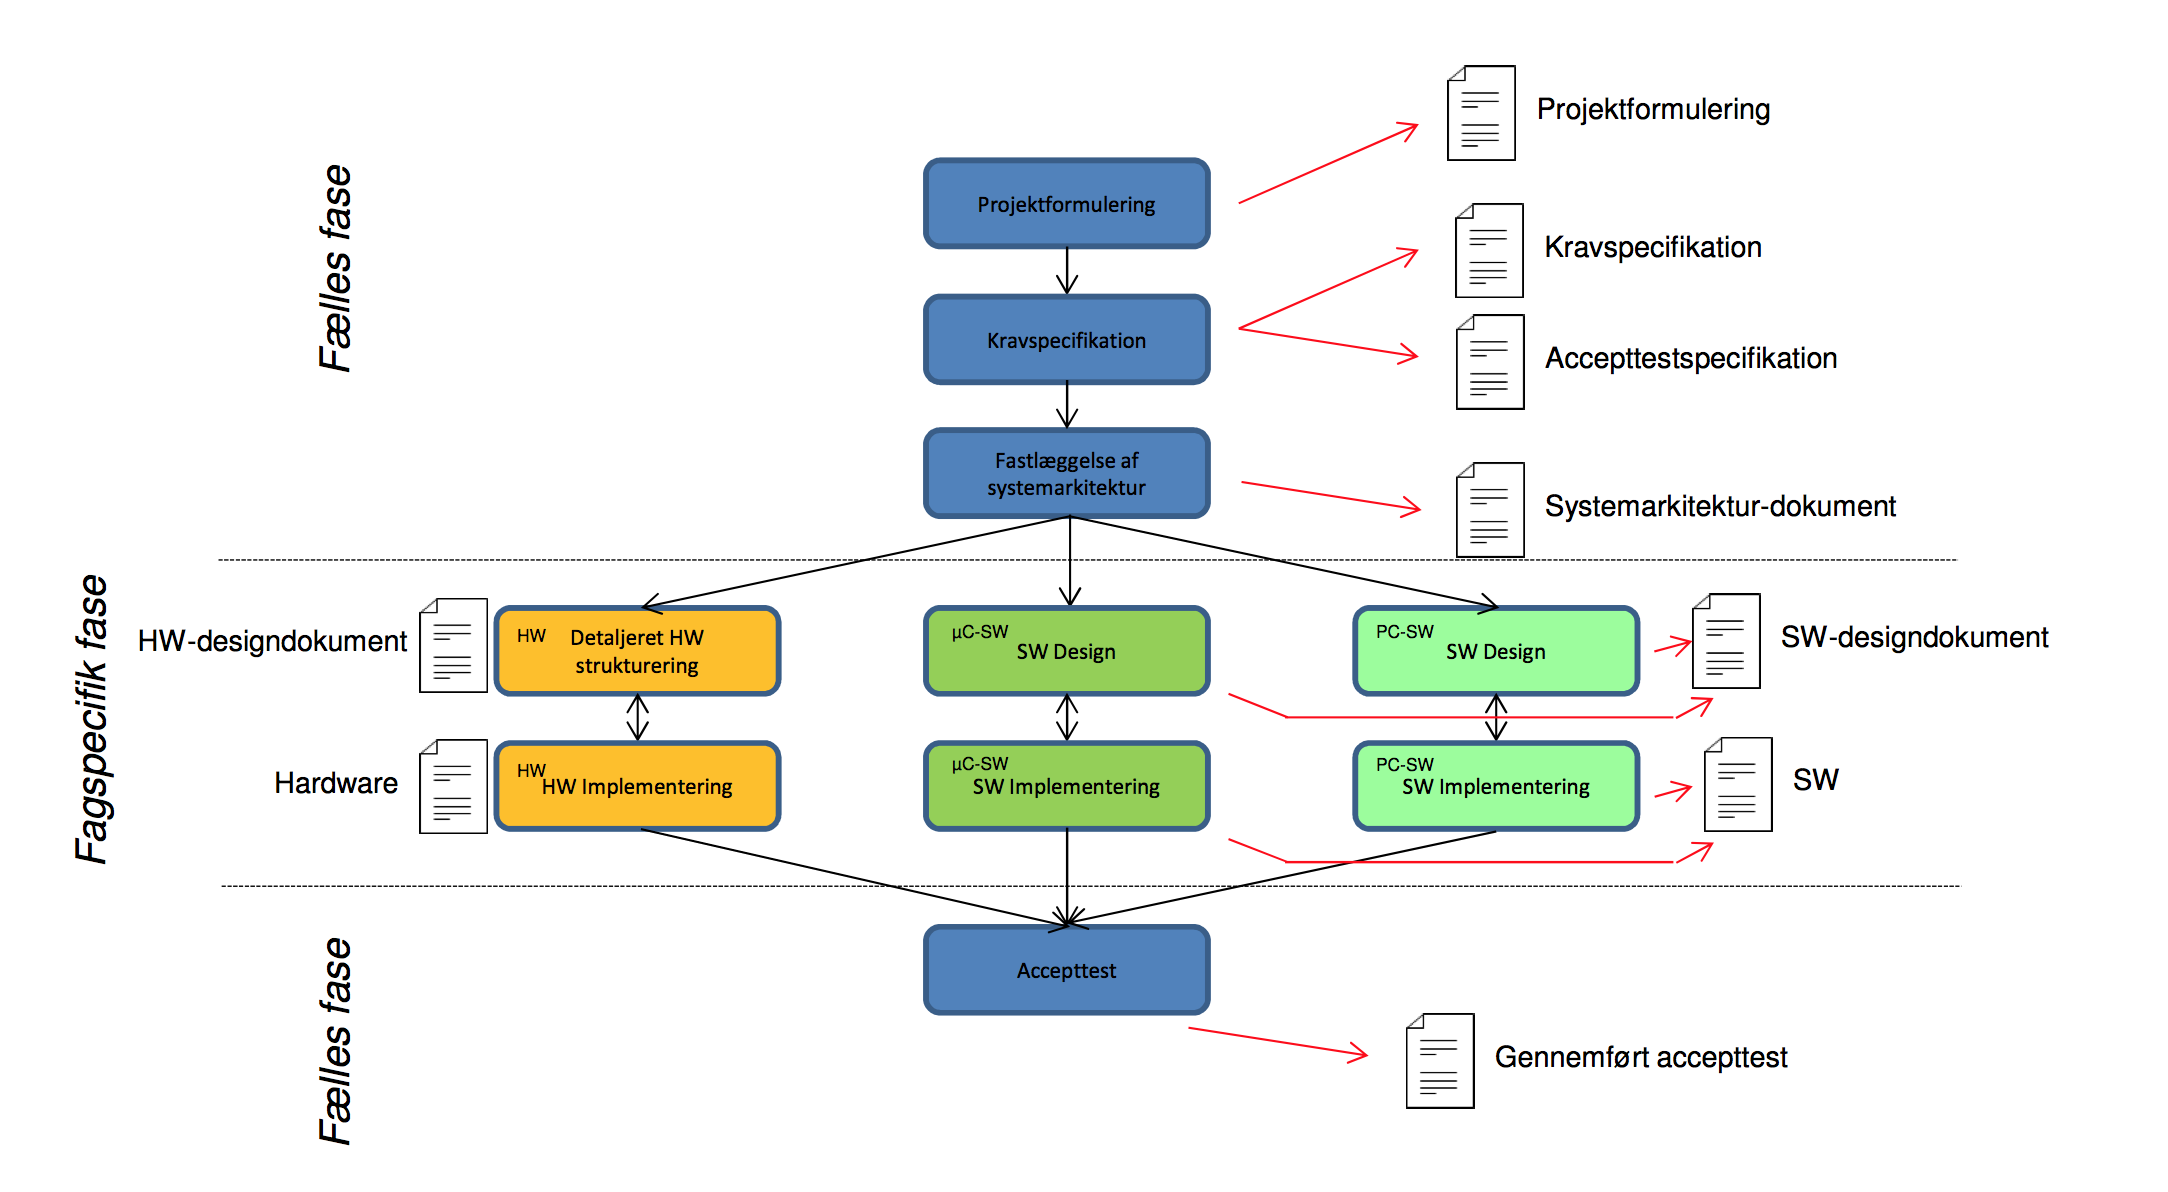
\includegraphics[width=0.8\textwidth]{billeder/ASE-modellen}
    \caption{ASE-modellen}
    \label{fig:ASE_model}
\end{figure}

I fællesfasen arbejde hele gruppen sammen omkring udarbejdelse af de forskellige deldokumenter. 
I den fagspecifikkefase deles gruppen op i mindre teams for at udvikle de fagspecifikke deldokumenter. 

ASE-modellen tager udgangspunkt i V-modellen (se figur XX).   

\begin{figure}[htbp]
  \centering
    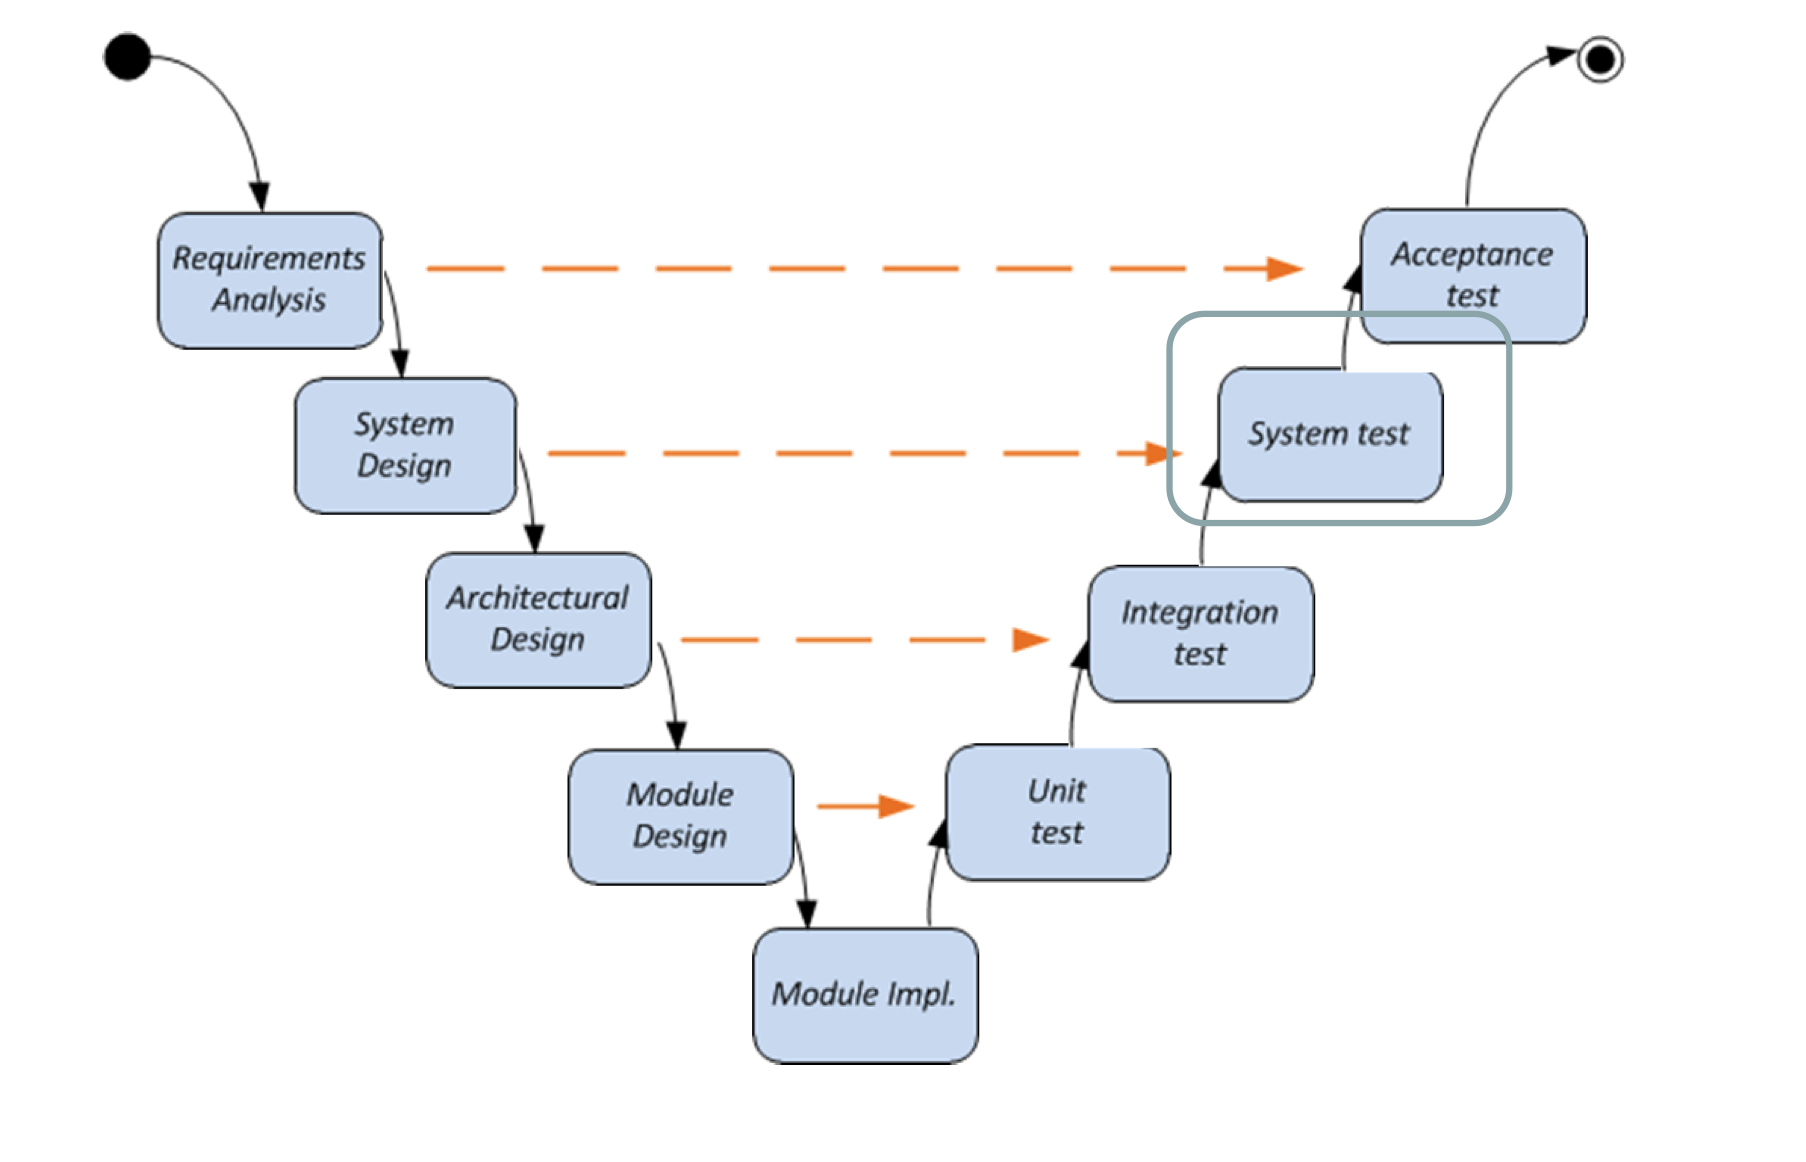
\includegraphics[width=0.8\textwidth]{billeder/V-modellen}
    \caption{V-modellen}
    \label{fig:V_model}
\end{figure}




\section{Møder, tidsplan, logbog og referater}

I forbindelse med projektforløbet er der afholdt en række møder. Vejledermøder, gruppemøder samt reviewmøder.

Vejledermøder er forbindelsen mellem gruppen og gruppens vejleder. Her har det været muligt at få foreløbelig feedback samt et indblik i om det der forventes også er det gruppen forventer. Afholdinngen af vejledermøder har været fastlagt til én i ugen. Det er næsten opretholdt, dog med enkelte aflysninger.

Gruppen har hver uge holdt mindst et, nogle gange flere møder. Disse møder er brugt til at afklare uoverensstemmelser og planlægning af den kommende uge. Under gruppemøderne er der 2 gange brugt tid på en trivsels runde. Her har det været mulgit at give ris/ros til gruppen og eller enkelte. Gruppemøderne startede lidt løst, men dette blev hurtigt ændret til at have en fast mødeholder, som styrede mødets gang. Tidsplanen er under gruppemøderne blevet revideret, således at den altid var opdateret til vejledermøderne.

Gruppekontrakt - bilag - skal underskrives og scannes så?

Reviewmøder har fungere således at gruppen enten udførte review på en anden gruppen og herefter fremlagde dette. Omvendt modtog gruppen lignende review fra andre grupper. Disse review førte ofte til uklarheder, som gruppen herefter måtte tage stilling til i gruppemødet.

Alle møder blev ajur ført med logbog og mødereferat. Her har gruppen haft en fast sekretær. 


  

